% Los objetivos específicos de cada uno de los subproyectos participantes, enumerándolos brevemente, con claridad, precisión y de manera realista (acorde con la duración prevista del proyecto).
%
% En los subproyectos con dos investigadores principales, deberá indicarse expresamente de qué objetivos específicos se hará responsable cada uno de ellos.
%

\begin{figure}
\centering
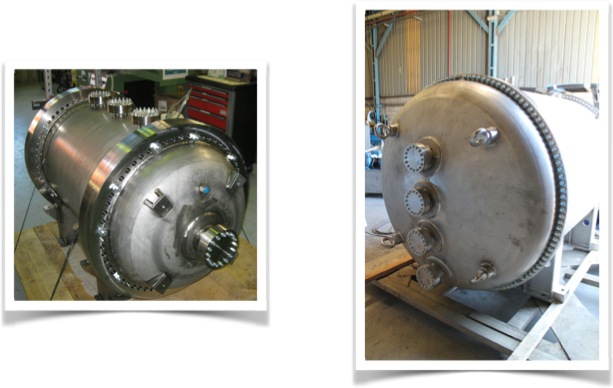
\includegraphics[height=8cm]{img/PV.png}
\caption{The NEW (left) and NEXT-100 (right) PV.} \label{fig:PV}
\end{figure}


\subsubsection*{Objectives of the COORD subproject}

The specific objectives of the COORD subproject are:

{\bf Construction of the NEW and NEXT-100 pressure vessels (WP1)}

The NEW and NEXT-100 pressure vessels, shown in Figure \ref{fig:PV} were designed to withstand pressures in excess of 20 bar, and to operate with negligible losses at 15 bar. They are built using a 316Ti alloy of low activity ($\sim$0.2 mBq/kg for the thorium series and 
the uranium series, as measured by our screening campaign). 
%The PVs have been payed from CUP funds. Inside the PVs an innder copper shielding (ICS) made of ultra pure copper bars of 6 cm (in the case of NEW) and 12 cm (in the case of NEXT-100) shield the gas volume from the residual radiation emitted by the lead shielding and the PV. The ICS of NEW will be payed by AdG funds. This project requires funding for the NEXT-100  ICS

The design of the PV was a collaboration between IFIC and LBNL groups. Manufacturing has involved several companies in Spain and has benefited from a CEDETI grant. The remaining activities in the project, which involves engineering personnel from IFIC and UPV is the construction and installation of the ICS for both NEW and NEXT-100, as well as the installation and commissioning of the PVs at the LSC.

{\bf Installation and commissioning of the Gas System for NEW and NEXT-100 at the LSC (WP2)}
 
The pressure vessel/gas system must be capable of pressurising, circulating, purifying, and depressurising the detector with xenon --- and in particular with very expensive enriched xenon (EXe) ---- argon and possibly other gases with negligible loss, and without damage to the detector. The probability of any substantial loss of EXe must be minimized. 

The most vulnerable component of the gas system is the re-circulation compressor.
The enriched \Xe\ used in NEXT 100 project is very expensive and therefore the compressor to move the gas through the re-circulation loop
must have sufficient redundancy to minimize the probability of failure and leakage. 
Furthermore, to preserve the purity of the gas all metal to metal seals must be used. A compressor manufactured by SERA satisfies this specifications \footnote{\texttt http://www.sera-web.com}.
This compressor is made with metal-to-metal seals on all the wetted surfaces. The gas is moved through the system by a triple stainless steel diaphragm. Between each
of the diaphragms there is a sniffer port to monitor for gas leakages. In the event of a leakage automatic emergency shutdown can be initiated.

As the xenon gas that will be used in the NEXT-100 is expensive, an automatic recovery system is needed
to evacuate the chamber in a case of an emergency condition. 

The gas system has been designed and extensively tested during the R\&D phase of the project. Furthermore, all the equipment (including the compressor, emergency recovery and recirculation loop) has been purchased using AdG/ERC funds.


{\bf  Construction of the infrastructures at LSC (WP3)}
The working platform, seismic pedestal and lead castle was designed by a collaboration between UPV and IFIC during 2012 and 2013 and the systems have been commissioned at the LSC in 2014. The remaining missing items are the radon suppression system and the clean tent. These system must be installed before starting operation of NEW (therefore in the second quarter of 2015 at latest). 

{\bf WP4: Construction of the field cage, light tube, HVFT and EL grids of NEW and NEXT-100}

The field cage (FC) produces an uniform electric ($\sim$ 300 V/cm) field inside the NEXT detectors that drifts the ionisation electron to the anode, where they are further accelerated in the electric field produced between a pair of transparent grids, called the electroluminescent (EL) grids. 

The main body of the field cage is a high density polyethylene (HDPE) cylindrical shell with a 2.5\,cm wall thickness.  The drift region will consist of OFHC copper strips connected with low background resistors.  The light tube consists of thin sheets of teflon, coated with tetraphenyl butadiene (TPB) wavelength shifter to shift the UV light produced in xenon to the blue region, around 450 nm.  A high-voltage feedthrough (HVFT) in the cathode and another one in the anode, allow the definition of the voltages. The cathode HVFT is designed to withstand up to 100 kV, and the HVFT of the anode to withstand up to 40 kV. The design of the HVFT, identical for NEW and NEXT-100 improve those that were built for DEMO by the Texas A\&M group. The field cage and grids of NEW and NEXT-100 are also identical, to a scale 1:2. The grids use a stainless steel mesh with pitch 0.5 mm and wire diameter 30 microns, which results in an open area of 90\%. Except for the size, the grids of NEW and NEXT-100 are also identical.   

The design of the FC, HVFT and grids is a collaboration between the USA groups and the IFIC group. The construction of the system for NEW is being carried out as a collaboration between IFIC (which is building the body of the FC in Spain) and the Texas groups, which are building the grids and the HVFTs. NEXT-100 FC will be built in the same way. 

{\bf Construction of the NEW/NEXT-100 energy planes (WP5)}

The energy measurement will be provided by the detection of EL light via PMTs, which will also record the scintillation light needed for $t_0$. Those PMTs will be located behind a transparent cathode.

%%%%%
\begin{figure}[t!b!]
\begin{center}
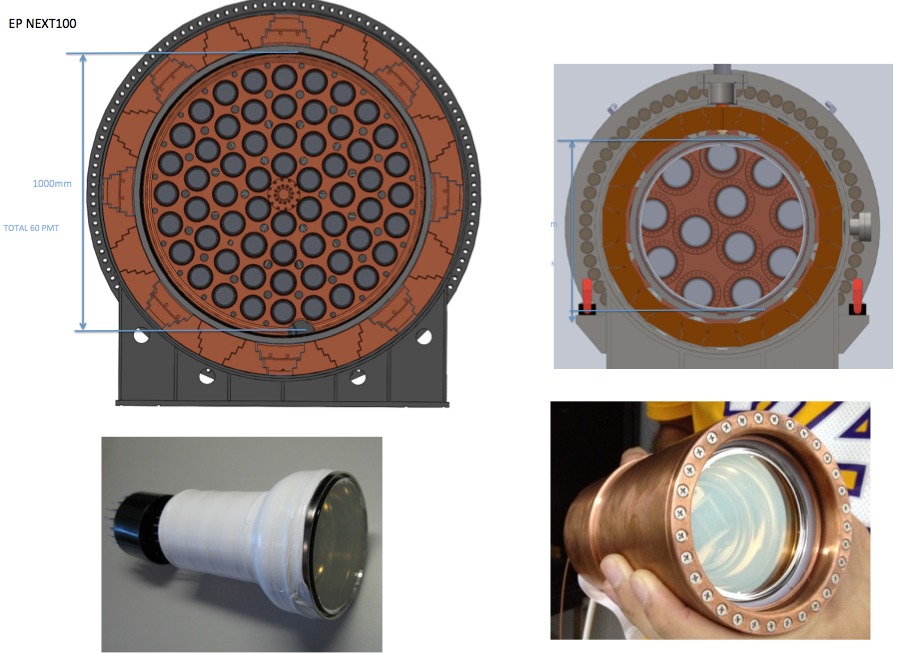
\includegraphics[width=.9\textwidth]{img/EPNext-100.png}
\end{center}
\caption{Top left: NEXT-100 energy plane (60 PMTs). Top right: NEW energy plane (12 PMTs).
Bottom left: The R11410-10 PMT from Hamamatsu; bottom right: a PMT can.} \label{fig:EnergyPlane}
\end{figure}
%%%%%


A total of 60 low-background, high-QE PMTs, model R11410-10 from Hamamatsu covering 32.5\% of the cathode area constitute the energy plane of NEXT-100 (Figure \ref{fig:EnergyPlane}, left). The R11410-10 are large tubes, with a 3'' photocathode and low levels of  activity of the order of 1 mBq per unit in the Uranium and Thorium series. The QE of the R11410-10 model is around 25\% both in the VUV and in the blue region. The  PMT coverage is 33\%, enough to guarantee detection of S1 in most of the energy spectrum and to measure the energy with good resolution.

PMTs are sealed into individual pressure resistant, vacuum tight copper enclosures (cans) coupled to 
sapphire windows. The cans are all connected via individual pressure resistant, vacuum tight tubing conduits to a central manifold. The PMT system is maintained at vacuum.

The NEW energy plane (Figure \ref{fig:EnergyPlane}, right) is currently under construction at IFIC. With 12 PMT cans (20\% of NEXT-100 sensors) it needs to cover an area of about half the radius, and provides therefore the same coverage. The NEXT-100 energy plane will be built also at IFIC. Construction will start immediately after the NEW engineering run, and will benefit from the methodology currently being developed for NEW, which includes: a) testing of PMTs; b) manufacturing of PMT cans; c) brazing of sapphire windows to PMT cans; d) cleaning and coating with TPB of PMT cans; e) coupling of PMTs to window, using certified optical glue; f) installation of cans in the vacuum-tight, support plate. 

%
 {\bf  Construction of the NEW/NEXT-100 tracking planes (WP6)}:

%%%%%%
\begin{figure}[tbhp!]
\begin{center}
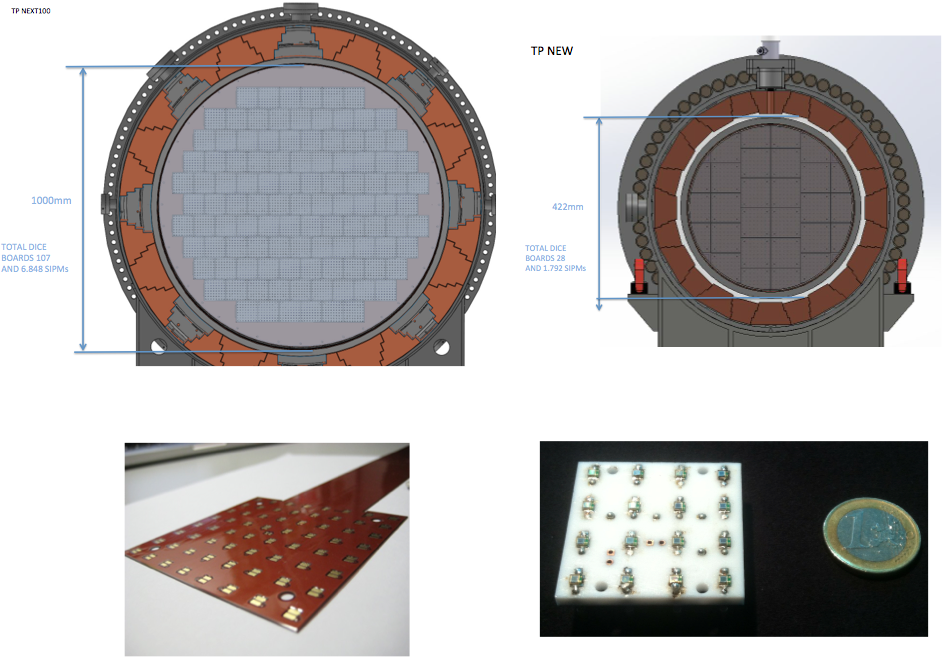
\includegraphics[width=0.7\textwidth]{img/TPNext-100.png}
\end{center}
\caption{Top left: the tracking plane of NEXT-100, will deploy 107 of the newly developed Kapton Dice Boards (KDB) shown in bottom left (64 SiPM per KDB, no connector, low noise tracing, low radioactivity). Top right: NEW will deploy about 20\% of the KDBs (28). Bottom right: the Cuflon Dice Board containing 16 (4$\times$4) SiPMs used for DEMO. The KDB improves dramatically the technology.} 
\label{fig.db2}
\end{figure}
%%%%%%

In NEXT the tracking function is provided by a plane of multi-pixel photon counters (MPPCs or SiPMs) operating as a light-pixels and located behind the transparent EL grids. The MPPCs will be manufactured by Hamamatsu and the chosen model is S10362-11-050P. This small device has an area of 1mm$^2$, 400 pixels per sensor and very large 
particle detection efficiency (PDE) in the blue region, close to 50\%. We have measured the spread in gain between the sensors to be less than 4\%, while the average in gain is (2.27 - 2.50) $\times10^5$. These values provide a homogeneous response of the plane, and ensure the correct resolution for the reconstruction of \bb\ events. Last but not least, MPPCs are very cost effective and its activity is very low, given its composition (mainly silica) and  light mass. 

The MPPCs are mounted in Dice Boards (DB). The original design, used for NEXT-DEMO, was based in   {\em cuflon} (PTFE fixed to a copper back plane) boards. During 2012 and 2013, a more advanced design, based in Kapton Dice Boards (KDBs) has been developed and fully tested. The KDBs host 65 SiPMs (rather than 16), are much more radipure than the  cuflon DB, since they have no connector, and introduce less electronic noise thanks to better routing of traces. 

Figure \ref{fig.db2} shows the tracking plane of NEXT-100 and that of NEW, together with the KDBs and the original cuflon DB. The tracking plane of NEW is also being manufactured at IFIC, and the tracking plane of NEXT-100 will follow the same protocol consisting in: a) production of KDBs; b) testing of KDB functionality; c) cleaning and mounting in the tracking plane support plate. 

{\bf Monte Carlo, Reconstruction and Software (WP11-WP13)}: During the R\&D phase the collaboration has developed a GEANT-4 based, full simulation of the various NEXT detectors (DEMO, DBDM, NEW and NEXT-100). In addition, the algorithms to reconstruct the topological signature and measure the energy of the event have been developed and tested with DEMO data. The offline reconstruction framework chosen in {\bf art}, a standard packaged developed and maintained at Fermilab (USA), as a part of the on-going collaboration with the USA groups. 